\section{One level: the Mermin--Peres square on the triangle}\label{sec:construction}

This section builds a single substitution step $S_\lambda$ from the Mermin--Peres square and analyzes its first application to the triangle $K_3$. Everything here uses only projective measurements on two qubits and elementary combinatorics, without topology.

\subsection{Six bases and nine shared planes}\label{sec:square}

We use the following realization of the Mermin--Peres square~\cite{Mermin,Peres}. Each entry in the table below lists the four coordinates of an unnormalized vector in $\C^4$, with $+$ and $-$ denoting $1$ and $-1$. In basis $i\in\{1,\ldots,6\}$, write $Q^i_s$ for the orthogonal projection onto the ray spanned by the vector listed under $s$. We call $s\in\{0,1,2,3\}$ a \emph{position}.
\[
\begin{array}{c|cccc}
 i\backslash s&0&1&2&3\\ \hline
 1& ++++ & +-+- & ++-- & +--+\\
 2& +000 & 0+00 & 00+0 & 000+\\
 3& +++- & ++-+ & +-++ & -+++\\
 4& +0+0 & +0-0 & 0+0+ & 0+0-\\
 5& ++00 & +-00 & 00++ & 00+-\\
 6& +00+ & +00- & 0++0 & 0+-0
\end{array}
\]
For each $r\in\{1,2,3\}$, set $A_r=\{0,r\}$ and $P^i_r=Q^i_0+Q^i_r$. Computing the spans of the corresponding pairs of rays yields the nine plane identities
\begin{equation}\label{eq:planes}
\begin{array}{ccc}
 P^1_1=P^4_2,&P^1_2=P^5_2,&P^1_3=P^6_2,\\
 P^2_1=P^5_1,&P^2_2=P^4_1,&P^2_3=P^6_1,\\
 P^3_1=P^5_3,&P^3_2=P^4_3,&P^3_3=I-P^6_3 .
\end{array}
\end{equation}
The six bases therefore form the two sides $\{1,2,3\}$ and $\{4,5,6\}$ of the complete bipartite graph $K_{3,3}$, which is the intersection graph of the square~\cite[Example~20]{Arkhipov}. We call bases $1,2,3$ the \emph{row bases} and bases $4,5,6$ the \emph{column bases}; the array~\eqref{eq:pauli-square} below gives the reason. We write an edge of this $K_{3,3}$ as $e=ik$ with $i\le3<k$. For such an edge, let $P_e$ be the projection on the left of its identity in~\eqref{eq:planes}, and call the range of $P_e$ the \emph{plane} of $e$.

Each of the two bases of an edge contains two rays that span its plane. For an end $b\in\{i,k\}$ of $e$, write $A_{b,e}$ for the set of the two positions of basis $b$ whose rays span the plane of $e$. Table~\ref{tab:edges} lists these sets. By~\eqref{eq:planes}, each of them is one of the sets $A_1,A_2,A_3$, with a single exception: the last identity equates $P^3_3$ with the complement of $P^6_3$, so that $A_{3,36}=A_3$ and $A_{6,36}=A_3^c=\{1,2\}$. We call $36$ the \emph{complemented edge} of $K_{3,3}$. Each of the eighteen projections $P^b_r$ appears exactly once in~\eqref{eq:planes}, with $P^6_3$ appearing through its complement. Thus the three edges of $K_{3,3}$ at a basis $b$ use the position sets $A_1,A_2,A_3$ once each if $b\le5$, and the sets $A_1,A_2,A_3^c$ if $b=6$.

\begin{table}[htbp]
\centering
\small
\begin{tabular}{@{}clll@{}}
\toprule
Edge $e=ik$ & Observable & $A_{i,e}$, at the row basis $i$ & $A_{k,e}$, at the column basis $k$ \\
\midrule
$14$ & $X\otimes I$ & $A_1=\{0,1\}$ & $A_2=\{0,2\}$ \\
$15$ & $I\otimes X$ & $A_2=\{0,2\}$ & $A_2=\{0,2\}$ \\
$16$ & $X\otimes X$ & $A_3=\{0,3\}$ & $A_2=\{0,2\}$ \\
$24$ & $I\otimes Z$ & $A_2=\{0,2\}$ & $A_1=\{0,1\}$ \\
$25$ & $Z\otimes I$ & $A_1=\{0,1\}$ & $A_1=\{0,1\}$ \\
$26$ & $Z\otimes Z$ & $A_3=\{0,3\}$ & $A_1=\{0,1\}$ \\
$34$ & $X\otimes Z$ & $A_2=\{0,2\}$ & $A_3=\{0,3\}$ \\
$35$ & $Z\otimes X$ & $A_1=\{0,1\}$ & $A_3=\{0,3\}$ \\
$36$ & $Y\otimes Y$ & $A_3=\{0,3\}$ & $A_3^c=\{1,2\}$ \\
\bottomrule
\end{tabular}
\caption{The nine edges of $K_{3,3}$. The plane of an edge $e=ik$ is the $+1$ eigenspace of the listed observable, which is the entry of~\eqref{eq:pauli-square} in row $i$ and column $k$. It is spanned by the rays of basis $i$ at the positions in $A_{i,e}$ and by the rays of basis $k$ at the positions in $A_{k,e}$. Only the last row contains a complement.}
\label{tab:edges}
\end{table}

To identify these projections with two-qubit Pauli observables, order the computational basis of $\C^4=\C^2\otimes\C^2$ as $00,01,10,11$ and let $X,Y,Z$ denote the Pauli matrices. Consider the array
\begin{equation}\label{eq:pauli-square}
\begin{array}{c|ccc}
 &\text{basis }4&\text{basis }5&\text{basis }6\\ \hline
\text{basis }1& X\otimes I& I\otimes X& X\otimes X\\
\text{basis }2& I\otimes Z& Z\otimes I& Z\otimes Z\\
\text{basis }3& X\otimes Z& Z\otimes X& Y\otimes Y
\end{array}
\end{equation}
whose rows are labeled by the row bases and whose columns by the column bases. Each basis is the joint eigenbasis of the three observables in its row or column, and for every edge $e=ik$ of $K_{3,3}$ the projection $P_e$ projects onto the $+1$ eigenspace of the observable in row $i$ and column $k$. The three observables in each row and in each of the first two columns multiply to $+I$, while those in the third column multiply to $-I$. This sign explains why the $+1$ eigenspace of $Y\otimes Y$ occupies $A_3$ in basis $3$ and $A_3^c$ in basis $6$.

The complemented identity in~\eqref{eq:planes} produces a parity obstruction to choosing a consistent ray in every basis.

\begin{lemma}[Parity of the square]\label{lem:parity}
There is no choice of one position $\sigma(i)\in\{0,1,2,3\}$ in each basis $i$ such that, for every edge $e=ik$ of $K_{3,3}$,
\[
 \sigma(i)\in A_{i,e}\quad\Longleftrightarrow\quad \sigma(k)\in A_{k,e}.
\]
\end{lemma}
\begin{proof}
Suppose such a function $\sigma$ exists, and count the pairs $(b,e)$ consisting of a basis $b\in\{1,\ldots,6\}$ and an incident edge $e$ of $K_{3,3}$ with $\sigma(b)\in A_{b,e}$.
\begin{itemize}
\item For each $b\in\{1,\ldots,5\}$, the three incident position sets are $A_1,A_2,A_3$. The position $\sigma(b)$ lies in all three sets if $\sigma(b)=0$, and in exactly one of them if $\sigma(b)\in\{1,2,3\}$. In either case basis $b$ contributes an odd number of pairs.
\item For $b=6$, the three incident position sets are $A_1,A_2,A_3^c$. The position $\sigma(6)$ lies in two of them if $\sigma(6)\in\{0,1,2\}$, and in none of them if $\sigma(6)=3$. Thus basis $6$ contributes an even number of pairs.
\end{itemize}
Summing over the six bases gives an odd total number of pairs. Under the equivalence in the lemma, however, each of the nine edges $e=ik$ of $K_{3,3}$ contributes either zero or two pairs, giving an even total. This contradiction proves the lemma.
\end{proof}

Each choice $\sigma(i)$ selects a ray of basis $i$, and the equivalence in Lemma~\ref{lem:parity} requires the rays chosen in two intersecting bases to lie on the same side of their shared plane. Such a choice would assign each of the nine observables in~\eqref{eq:pauli-square} a basis-independent value $\pm1$, which is the Kochen--Specker contradiction of the square in the form of Mermin and Peres~\cite{KS,Mermin,Peres}.

\subsection{A worked example: from the triangle to level two}\label{sec:example}

Before stating the general substitution, we inspect its first application to the triangle $K_3$ without intermediate wire layers---the graph $S_0(K_3)$---and one vertex at level two. In this subsection we label the three vertices of $K_3$ by the colors $\col r,\col g,\col b$.

\paragraph{Vertices, words, and measurements.}
A vertex of $S_0(K_3)$ is a pair $(i,g)$ consisting of a basis $i\in\{1,\ldots,6\}$ and a \emph{word} $g=g_0g_1g_2g_3\in\{\col r,\col g,\col b\}^4$ whose first letter $g_0$ repeats at least once among $g_1,g_2,g_3$. When the referee sends $(i,g)$, the player measures basis $i$, obtains a position $s\in\{0,1,2,3\}$, and answers with the color $g_s$. The \emph{measurement} of the vertex is therefore the three-outcome projective measurement whose projector for a color $a$ is the sum of $Q^i_s$ over all positions $s$ with $g_s=a$. We keep three notions distinct: the vertex is the pair $(i,g)$, its word is $g$, and its measurement may coincide with the measurement of other vertices. For each of the three choices of $g_0$, exactly $2^3$ words avoid $g_0$ in the remaining three positions, so there are $3^4-3\cdot2^3=57$ admissible words per basis and $6\cdot57=342$ vertices in $S_0(K_3)$.

\paragraph{Edges inside a basis.}
Two vertices in the same basis are adjacent precisely when their words differ in all four positions, such as $\col{rrgb}$ and $\col{ggbr}$. Players who receive two such vertices measure the same basis on their shared maximally entangled state and obtain the same position $s$, where their words specify distinct colors. Equivalently, for every color $a$, the two projectors for $a$ sum $Q^i_s$ over disjoint sets of positions and are therefore orthogonal.

\paragraph{Edges between bases.}
A row basis $i$ and a column basis $k$ share the plane of the edge $e=ik$ of $K_{3,3}$. A word of basis $i$ that takes a single color $x$ on $A_{i,e}$ and a single color $y$ on $A_{i,e}^c$ depends only on whether the measured ray lies in the plane of $e$. The same holds for a word of basis $k$ taking color $x'$ on $A_{k,e}$ and color $y'$ on $A_{k,e}^c$. We join these two vertices by an edge whenever $x\ne x'$ and $y\ne y'$. Both players then obtain the same binary outcome for $\{P_e,I-P_e\}$ and return different colors in either case.

\paragraph{The complemented edge of $K_{3,3}$.}
On eight edges of $K_{3,3}$, the shared plane occupies a position set of the form $\{0,r\}$ in both bases. On the edge $e=36$, which joins bases $3$ and $6$, the $+1$ eigenspace of $Y\otimes Y$ occupies positions $\{0,3\}$ in basis $3$ and positions $\{1,2\}$ in basis $6$. Consider the two vertices
\[
 u=(3,\col{rggr}),\qquad
 v=(6,\col{rggr}).
\]
On the plane $P_{36}$, vertex $u$ returns $\col r$ whereas vertex $v$ returns $\col g$. On its orthogonal complement $I-P_{36}$, vertex $u$ returns $\col g$ whereas vertex $v$ returns $\col r$. Hence $u$ and $v$ are adjacent even though their words coincide. Conversely, $(6,\col{grrg})$ and $u$ are distinct vertices with different words that carry the same measurement, since both return $\col r$ on $P_{36}$ and $\col g$ on $I-P_{36}$.

\paragraph{Tagged and physical graphs.}
Because $S_0(K_3)$ keeps a separate vertex for each pair $(i,g)$, we call it a \emph{tagged} graph: each vertex remembers the presentation of its measurement (here its basis, and below also a wire and a layer). A graph whose vertices are distinct projective measurements and whose edges join every pair of measurements that are orthogonal at every outcome is called \emph{physical}. Our main families are tagged, because separating distinct presentations of the same measurement allows graph distance to control commutation. By contrast, the physical graph $F_{\rm phys}$ in Section~\ref{sec:165} selects $39$ of the $57$ words per basis and has $165$ vertices.

Merging the vertices of $S_0(K_3)$ that carry identical measurements leaves $273$ distinct measurements. Indeed, the $3$ constant words give the same measurement in all six bases. Each basis has $18$ further words that take one color on some $A_r$ and another on $A_r^c$. They give $6$ measurements for each of the nine planes, $9\cdot6=54$ in all. Each of these is shared by the two bases of its edge and by no third basis, because the nine observables in~\eqref{eq:pauli-square} differ pairwise even up to sign. The remaining $57-3-18=36$ words of a basis have a color that occurs at a single position. Their measurements therefore contain a projection onto one ray, and they determine the basis, because the $24$ rays of the six bases are distinct. They give $6\cdot36=216$ measurements. In total, $3+54+216=273$.

\paragraph{A vertex of level two.}
At level two, the four entries of a word are themselves vertices of $S_0(K_3)$. Using the vertices $u$ and $v$ above, we can form
\[
 w=\bigl(6,(u,v,v,u)\bigr).
\]
A player receiving $w$ first measures basis $6$ on the first two-qubit register. Positions $0$ and $3$ select $u$, instructing the player to measure basis $3$ on the second register; positions $1$ and $2$ select $v$, instructing the player to measure basis $6$ on the second register. In either case the selected word $\col{rggr}$ determines the final color. The resulting three-outcome measurement acts on $\C^4\otimes\C^4$.

\subsection{The square substitution and its quantum strategy}\label{sec:substitution}

To increase the compatibility radius beyond $2$, we stretch each edge of $K_{3,3}$ into a multi-layer wire so that distinct bases sit at least $\lambda+1$ steps apart.

For a finite simple graph $H$ and an integer $\lambda\ge0$, the \emph{square substitution} $S_\lambda(H)$ is the graph defined by the following three rules.
\begin{itemize}
\item \emph{Basis charts.} For each basis $i\in\{1,\ldots,6\}$, take a separately labeled copy of the set of words
\[
 (g_0,g_1,g_2,g_3)\in V(H)^4,\qquad
 g_0=g_r\ \text{for some }1\le r\le3.
\]
This set is the \emph{basis chart} at $i$. Two words in the same basis chart are adjacent precisely when their entries are adjacent in $H$ in all four positions.
\item \emph{Wires.} Along each edge $e=ik$ of $K_{3,3}$ (with $i\le3<k$), place a \emph{wire} consisting of \emph{layers} $\ell=0,\ldots,\lambda+1$, each a copy of $V(H)^2$. Within a wire, two vertices $(x,y)$ and $(x',y')$ in equal or consecutive layers are adjacent whenever $x\sim_H x'$ and $y\sim_H y'$.
\item \emph{Identifications.} Identify each pair $(x,y)$ in layer $0$ of the wire along $e$ with the word in basis chart $i$ that takes $x$ on $A_{i,e}$ and $y$ on $A_{i,e}^c$. Identify each pair $(x,y)$ in layer $\lambda+1$ with the word in basis chart $k$ that takes $x$ on $A_{k,e}$ and $y$ on $A_{k,e}^c$. No other identifications are made. The vertices in the $\lambda$ \emph{interior} layers $\ell=1,\ldots,\lambda$ retain their wire and layer labels $(e,\ell,x,y)$.
\end{itemize}
For $\lambda=0$, layers $0$ and $1$ are consecutive and connect the two endpoint sets directly, which reproduces $S_0(K_3)$ from Section~\ref{sec:example}. Figure~\ref{fig:wire} illustrates the wire on the complemented edge $36$ of $K_{3,3}$ for $H=K_3$ and $\lambda=1$.

\begin{figure}[htbp]
\centering
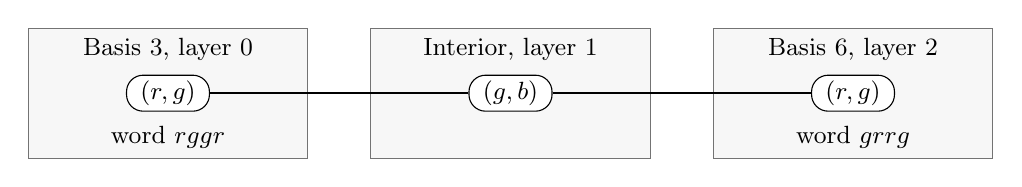
\begin{tikzpicture}[x=1cm,y=1cm,
    layer/.style={draw=black!55,fill=black!3,minimum width=3.55cm,minimum height=1.65cm},
    vertex/.style={draw=black,fill=white,rounded corners=6pt,inner xsep=5pt,inner ysep=2pt},
    every node/.style={font=\small}]
  \foreach \x in {-4.35,0,4.35} \node[layer] at (\x,0) {};
  \node at (-4.35,.56) {Basis 3, layer $0$};
  \node at (0,.56) {Interior, layer $1$};
  \node at (4.35,.56) {Basis 6, layer $2$};
  \node[vertex] (left) at (-4.35,0) {$(\col r,\col g)$};
  \node[vertex] (middle) at (0,0) {$(\col g,\col b)$};
  \node[vertex] (right) at (4.35,0) {$(\col r,\col g)$};
  \draw[semithick] (left.east)--(middle.west) (middle.east)--(right.west);
  \node at (-4.35,-.56) {word $\col{rggr}$};
  \node at (4.35,-.56) {word $\col{grrg}$};
\end{tikzpicture}
\caption{The wire between bases $3$ and $6$ for $H=K_3$ and $\lambda=1$. Each box holds nine vertices, one for every ordered pair of colors. The three marked vertices form a path because both entries change across each drawn edge. At the endpoints, the first entry of $(\col r,\col g)$ occupies positions $\{0,3\}$ in basis $3$ and $\{1,2\}$ in basis $6$. The two endpoint vertices are the vertex $u$ of Section~\ref{sec:example} and the vertex in basis $6$ carrying the same measurement.}
\label{fig:wire}
\end{figure}

We now lift any quantum $3$-coloring of $H$ to $S_\lambda(H)$ at a factor-of-four cost in local dimension. Let $(P_{x,a})_{a\in\mathbb Z/3}$, for $x\in V(H)$, be a quantum $3$-coloring of $H$ on $\C^d$; we call it the input coloring. Its \emph{lift} consists of projectors $P'_{v,a}$ on $\C^4\otimes\C^d$. At a basis word $(i,g)$ and at a wire vertex $(e,\ell,x,y)$, define
\begin{equation}\label{eq:strategy}
 P'_{(i,g),a}=\sum_{s=0}^3 Q^i_s\otimes P_{g_s,a},
 \qquad
 P'_{(e,\ell,x,y),a}
 =P_e\otimes P_{x,a}+(I-P_e)\otimes P_{y,a}.
\end{equation}
Operationally, the first formula measures basis $i$ on $\C^4$ and then applies the measurement of the selected entry $g_s$ on $\C^d$; the second measures the binary plane observable $\{P_e,I-P_e\}$ and applies the measurement of $x$ or $y$ accordingly. By~\eqref{eq:planes} and the definition of $A_{b,e}$, the two formulas agree at every wire endpoint, including both ends of the complemented edge $36$ of $K_{3,3}$. Each formula defines a projective measurement because its first-factor projections are pairwise orthogonal and sum to $I$. On an edge inside a basis chart, the edge rule $P'_{(i,g),a}P'_{(i,g'),a}=0$ holds separately in each of the four orthogonal summands $Q^i_s$; on a wire edge, it holds separately on the range and kernel of $P_e$.

The next lemma shows that~\eqref{eq:strategy} preserves $R$-compatibility whenever $R\le\lambda+2$.

\begin{lemma}\label{lem:radius-lift}
If the coloring of $H$ is $R$-compatible and $R\le\lambda+2$, then~\eqref{eq:strategy} gives an $R$-compatible quantum $3$-coloring of $S_\lambda(H)$.
\end{lemma}
\begin{proof}
Let $u,v\in V(S_\lambda(H))$ satisfy $\dist_{S_\lambda(H)}(u,v)\le R$, and fix a shortest path $\gamma$ of length at most $R$ between $u$ and $v$. For a basis $b$, a \emph{wire at $b$} is a wire along an edge of $K_{3,3}$ that contains $b$. Its vertices include those of both end layers, also the ones that are identified with words of the other basis chart. We claim that there is a basis $b\in\{1,\ldots,6\}$ such that every vertex of $\gamma$ lies in basis chart $b$ or on a wire at $b$. There are three cases, according to the number of basis charts that $\gamma$ visits.
\begin{itemize}
\item If $\gamma$ visits no basis chart, all its vertices lie in the interior of a single wire $e$, because distinct wires meet only at basis charts. Either end of $e$ can serve as $b$.
\item If $\gamma$ visits exactly one basis chart, every wire met by $\gamma$ is a wire at the basis of that chart, and this basis is $b$.
\item Suppose that $\gamma$ visits at least two basis charts. Choose a minimal subpath of $\gamma$ that connects two distinct basis charts, with no chart vertex in between. It traverses a wire $e$ from layer $0$ to layer $\lambda+1$ and has at least $\lambda+1$ edges. Since $\gamma$ has at most $R\le\lambda+2$ edges, at most one edge of $\gamma$ lies outside this subpath.
  \begin{itemize}
  \item If there is no such edge, all vertices of $\gamma$ lie on $e$, and either end of $e$ can serve as $b$.
  \item If there is one, it is attached to one end of the subpath. Let $b$ be the basis at that end. The additional vertex is adjacent to a word of basis chart $b$, so it lies in basis chart $b$ or on a wire at $b$. For $\lambda=0$ and $R=2$ it may be a word of a third basis chart, at the far end of a second wire at $b$.
  \end{itemize}
\end{itemize}

This proves the claim. It implies that the measurement~\eqref{eq:strategy} of every vertex of $\gamma$ is diagonal in basis $b$ in the first tensor factor. Indeed, for any wire $e$ at $b$ we have $P_e=\sum_{s\in A_{b,e}} Q^b_s$ and $I-P_e=\sum_{s\notin A_{b,e}} Q^b_s$ by~\eqref{eq:planes}. Hence every vertex $w$ along $\gamma$ can be written in the form
\[
 P'_{w,a}=\sum_{s=0}^3 Q^b_s\otimes P_{\alpha_s(w),a},
\]
where $\alpha_s(w)\in V(H)$ is $g_s$ if $w=(b,g)$ lies in chart $b$, and equals $x$ for $s\in A_{b,e}$ and $y$ for $s\notin A_{b,e}$ if $w=(e,\ell,x,y)$ lies on a wire $e$ at $b$. Across every edge of $\gamma$, whether inside chart $b$ or along a wire at $b$, the adjacency rules of $S_\lambda(H)$ force $\alpha_s(w)\sim_H \alpha_s(w')$ at each fixed position $s\in\{0,1,2,3\}$. Therefore, for each $s$, the sequence of labels $\alpha_s(w)$ along $\gamma$ is a walk in $H$ of length at most $R$, so $\dist_H(\alpha_s(u),\alpha_s(v))\le R$. Because the input coloring of $H$ is $R$-compatible, $P_{\alpha_s(u),a}$ and $P_{\alpha_s(v),a'}$ commute for all outcomes $a,a'$ and every $s$. Since the four projections $Q^b_s$ are pairwise orthogonal, $P'_{u,a}$ and $P'_{v,a'}$ commute for all $a,a'$.
\end{proof}

For $H=K_3$, the input coloring consists of the \emph{scalar projectors} $P_{x,a}=\mathbf 1_{x=a}$ on $\C^1$ (local dimension $d=1$). Equation~\eqref{eq:strategy} then gives a strategy in local dimension $4$ that reproduces Section~\ref{sec:example}: at $(i,g)$, measure basis $i$ on two qubits and return the color $g_s$ at the obtained position $s$; at a wire vertex $(e,\ell,x,y)$, return $x$ on $P_e$ and $y$ on $I-P_e$.

\subsection{Five classical colors without topology}\label{sec:five}

We now show by a purely combinatorial argument that $\chi(S_\lambda(K_3))=5$ for every $\lambda\ge0$. The proof relies on three rigidity properties of proper $4$-colorings of the categorical powers $K_3^{\times2}$ and $K_3^{\times3}$, where vertices are pairs or triples of colors and two tuples are adjacent precisely when they differ in every coordinate.

Call the nine vertices of $K_3^{\times2}$ \emph{cells}, and arrange them in a $3\times3$ grid: three cells sharing their first coordinate form a \emph{row} of the grid, and three cells sharing their second coordinate form a \emph{column}. In any proper coloring of $K_3^{\times2}$, two cells of the same color must agree in at least one coordinate. Consequently, any color class containing two cells in the same row lies entirely in that row; we call such a color class a \emph{row class}, and define a \emph{column class} symmetrically. A proper coloring of $K_3^{\times2}$ \emph{reads the first coordinate} if some column consists entirely of cells belonging to row classes, and \emph{reads the second coordinate} if some row consists entirely of cells belonging to column classes. For example, the $3$-coloring $(x,y)\mapsto x$ reads the first coordinate.

\begin{lemma}[Four colors read one coordinate]\label{lem:four-colorings}
\leavevmode
\begin{enumerate}
\item[(a)] Every proper $4$-coloring of $K_3^{\times2}$ reads exactly one of the two coordinates.
\item[(b)] Let $f,g$ be proper colorings of $K_3^{\times2}$ with colors from the same set of four colors, such that $f(u)\ne g(v)$ whenever the cells $u,v$ differ in both coordinates. Then $f$ and $g$ read the same coordinate.
\item[(c)] Let $f$ be a proper $4$-coloring of $K_3^{\times3}$. For $m=1,2,3$, let $f_m(x,y)$ be the color of the triple with $x$ in coordinate $m$ and $y$ in the other two coordinates. Then exactly one of the three colorings $f_1,f_2,f_3$ of $K_3^{\times2}$ reads the first coordinate.
\end{enumerate}
\end{lemma}

The analytical proof of Lemma~\ref{lem:four-colorings} is given in Appendix~\ref{app:k3-four}. (Lemma~\ref{lem:four-colorings} is related to the case $t=3$ of~\cite[Lemma~3.7]{BG}, which is not imported here.)

For a basis $i$ and $\{r,s,t\}=\{1,2,3\}$, the partition $\{A_r,\{s\},\{t\}\}$ of the four positions, taken together with the basis $i$, is a \emph{ternary template} at basis $i$. Every basis has three ternary templates, so there are eighteen in all. In the basis chart of $S_\lambda(K_3)$ at $i$, the $27$ words that are constant on $A_r$ induce a copy of $K_3^{\times3}$ indexed by the three parts $A_r,\{s\},\{t\}$, because two such words differ in all four positions precisely when they take different colors on all three parts.

\begin{theorem}[One substitution]\label{thm:one-level}
For every $\lambda\ge0$, the graph $S_\lambda(K_3)$ has quantum chromatic number three, with a $(\lambda+2)$-compatible quantum $3$-coloring in local dimension four, and classical chromatic number five.
\end{theorem}

The idea of the lower bound is this. A proper $4$-coloring of $S_\lambda(K_3)$ would assign a single position $\sigma(i)$ to each basis and thereby assign every observable in~\eqref{eq:pauli-square} a basis-independent sign $\pm1$; the fifth color is what classical players need to evade this commitment. For three colors the obstruction is immediate, because every proper $3$-coloring of $K_3^{\times3}$ depends on a single coordinate (Appendix~\ref{app:k3-powers}).

\begin{proof}
We establish the quantum coloring, exclude classical $4$-colorings via Lemmas~\ref{lem:four-colorings} and~\ref{lem:parity}, and verify that five colors suffice.

\emph{Quantum $3$-coloring.} The scalar projectors on $K_3$ commute at every distance, so Lemma~\ref{lem:radius-lift} applied with $R=\lambda+2$ yields a $(\lambda+2)$-compatible quantum $3$-coloring of $S_\lambda(K_3)$ in local dimension four. The three constant words in any single basis chart form a triangle, so $\cq(S_\lambda(K_3))=3$.

\emph{Four colors do not suffice.} Suppose for contradiction that $f$ is a proper $4$-coloring of $S_\lambda(K_3)$. Let $D$ be any part of a ternary template, that is, one of the six sets $A_1,A_2,A_3,\{1\},\{2\},\{3\}$. For each basis $i\in\{1,\ldots,6\}$ and each pair $(x,y)\in V(K_3)^2$, let $f^i_D(x,y)$ be the color under $f$ of the word in basis chart $i$ that equals $x$ on $D$ and $y$ on $D^c$. Every such word is constant on at least one $A_r$ and therefore belongs to basis chart $i$. Pairs $(x,y)$ and $(x',y')$ differing in both coordinates yield words differing in all four positions, so $f^i_D$ is a proper $4$-coloring of $K_3^{\times2}$. We say that $f$ \emph{reads $D$ at basis $i$} if $f^i_D$ reads the first coordinate.

Fix a basis $i$. On the $27$ words constant on $A_r$ (forming a copy of $K_3^{\times3}$ for the ternary template $\{A_r,\{s\},\{t\}\}$), the three derived colorings of Lemma~\ref{lem:four-colorings}(c) are precisely $f^i_{A_r}$, $f^i_{\{s\}}$, and $f^i_{\{t\}}$. By Lemma~\ref{lem:four-colorings}(c), $f$ reads exactly one part of each of the three ternary templates at basis $i$:
\begin{itemize}
\item If $f$ reads some singleton $\{t\}$ ($t\in\{1,2,3\}$), then the two templates containing $\{t\}$ force $f$ to read none of $A_r,A_s,\{r\},\{s\}$, and the third template $\{A_t,\{r\},\{s\}\}$ forces $f$ to read $A_t$. Set $\sigma(i)=t$.
\item If $f$ reads no singleton, then each template forces $f$ to read its doubleton part, so $f$ reads $A_1$, $A_2$, and $A_3$. Set $\sigma(i)=0$.
\end{itemize}
In both cases, for all six sets $D\in\{A_1,A_2,A_3,\{1\},\{2\},\{3\}\}$,
\begin{equation}\label{eq:selected-position}
 f\text{ reads }D\text{ at basis }i\quad\Longleftrightarrow\quad \sigma(i)\in D.
\end{equation}

Now fix an edge $e=ik$ of $K_{3,3}$ (with $i\le3<k$). For each layer $\ell\in\{0,\ldots,\lambda+1\}$ of the wire along $e$, let $h_\ell(x,y)$ denote the color under $f$ of the vertex $(x,y)$ in layer $\ell$. Each $h_\ell$ is a proper $4$-coloring of $K_3^{\times2}$, and consecutive layers $h_\ell,h_{\ell+1}$ satisfy the cross-edge hypothesis of Lemma~\ref{lem:four-colorings}(b). By induction along the wire, $h_0$ and $h_{\lambda+1}$ read the same coordinate. At layer $0$, the endpoint identification gives $h_0=f^i_{A_{i,e}}$, so by~\eqref{eq:selected-position}
\[
 h_0\text{ reads the first coordinate}\quad\Longleftrightarrow\quad\sigma(i)\in A_{i,e}.
\]
Suppose first that $e\ne36$. Then $A_{k,e}=A_r$ for some $r$ and $h_{\lambda+1}=f^k_{A_{k,e}}$, so by~\eqref{eq:selected-position}
\[
 h_{\lambda+1}\text{ reads the first coordinate}\quad\Longleftrightarrow\quad\sigma(k)\in A_{k,e}.
\]
Now let $e=36$, so that $A_{6,36}=A_3^c$. The endpoint identification places $x$ on $A_3^c$ and $y$ on $A_3$, so $h_{\lambda+1}(x,y)=f^6_{A_3}(y,x)$. Thus $h_{\lambda+1}$ reads the first coordinate precisely when $f^6_{A_3}$ reads the second. By Lemma~\ref{lem:four-colorings}(a), this happens precisely when $f^6_{A_3}$ does not read the first coordinate, that is, by~\eqref{eq:selected-position}, when $\sigma(6)\notin A_3$. Hence
\[
 h_{\lambda+1}\text{ reads the first coordinate}\quad\Longleftrightarrow\quad\sigma(6)\in A_3^c=A_{6,36}.
\]
In both cases, since $h_0$ and $h_{\lambda+1}$ read the same coordinate, we obtain $\sigma(i)\in A_{i,e}$ if and only if $\sigma(k)\in A_{k,e}$, for every edge $e=ik$ of $K_{3,3}$. This contradicts Lemma~\ref{lem:parity}. Hence $\chi(S_\lambda(K_3))\ge5$.

\emph{Five colors suffice.} Mapping each vertex of $S_\lambda(K_3)$ to its projective measurement~\eqref{eq:strategy} gives a graph homomorphism into the physical graph of all three-label measurements formed from the six bases. Proposition~\ref{prop:physical-upper} in Appendix~\ref{app:five-coloring} (applied with $n=3$) properly colors that physical graph with five colors. Therefore $\chi(S_\lambda(K_3))=5$.
\end{proof}

\subsection{Generalizing to arbitrary triads}\label{sec:one-in-three}

The proof of Theorem~\ref{thm:one-level} uses nothing specific to two qubits beyond Lemma~\ref{lem:four-colorings} and the absence of a consistent choice of one ray per basis. We now isolate this mechanism for arbitrary sets of three-outcome projective measurements; Section~\ref{sec:alldim} applies it to Peres' $33$ rays in $\R^3$ to obtain graphs with $(\cq,\chi)=(3,5)$ admitting quantum $3$-colorings in local dimension three at every compatibility radius.

Let $\mathcal D$ be a finite nonempty set of \emph{triads}, where a triad is an unordered triple $\{E_1,E_2,E_3\}$ of nonzero orthogonal projections on $\C^d$ summing to $I$. We call $E_1,E_2,E_3$ the \emph{parts} of the triad. Because its three parts are nonzero and sum to $I$, a triad contains at most one member of any complementary pair $\{P,I-P\}$. A \emph{one-in-three selection} for $\mathcal D$ chooses exactly one part in every triad such that, across distinct triads, two equal parts are either both chosen or both unchosen, and of two complementary parts exactly one is chosen.

For an integer $\lambda\ge0$, the graph $W_\lambda(\mathcal D)$ is built from charts and wires in the same way as $S_\lambda(K_3)$.
\begin{itemize}
\item \emph{Charts.} Each triad $T\in\mathcal D$ has a \emph{chart} of $27$ words, which assign one of the three colors to each of its three parts. Two words of the same chart are adjacent whenever they differ on all three parts.
\item \emph{Wires.} For every complementary pair $\{P,I-P\}$ that occurs among the parts of $\mathcal D$, fix an ordering of the triads that contain $P$ or $I-P$. Let $T_1$ be the first of these triads, with part $P_1\in\{P,I-P\}$. The chart of $T_1$ is connected to the chart of every other triad $T$ in the list by a \emph{wire} of layers $\ell=0,\ldots,\lambda+1$, each a copy of $V(K_3)^2$. Within a wire, $(x,y)$ and $(x',y')$ in equal or consecutive layers are adjacent whenever $x\ne x'$ and $y\ne y'$.
\item \emph{Identifications.} The pair $(x,y)$ in layer $0$ is identified with the word of $T_1$ that assigns $x$ to $P_1$ and $y$ to the other two parts. The pair $(x,y)$ in layer $\lambda+1$ is identified with the word of $T$ that carries the same measurement: if $T$ contains $P_1$, this word assigns $x$ to $P_1$ and $y$ to the other two parts of $T$; if $T$ contains $I-P_1$, it assigns $y$ to $I-P_1$ and $x$ to the other two parts of $T$.
\item \emph{Measurements.} A chart word carries the projective measurement whose projector for a color $a$ is the sum of the parts colored $a$. A wire vertex $(x,y)$ carries the measurement that returns $x$ on $P_1$ and $y$ on $I-P_1$.
\end{itemize}
The graph $W_\lambda(\mathcal D)$ depends on the chosen orderings of the triads, but the following result holds for every choice.

\begin{proposition}[One-in-three configurations]\label{prop:one-in-three}
These measurements form a $(\lambda+2)$-compatible quantum $3$-coloring of $W_\lambda(\mathcal D)$ in local dimension $d$, and $\cq(W_\lambda(\mathcal D))=3$. If $\mathcal D$ has no one-in-three selection, then $\chi(W_\lambda(\mathcal D))\ge5$.
\end{proposition}
\begin{proof}
\emph{Edge rule and $\cq=3$.} On a chart edge, the two projectors for any fixed color $a$ sum over disjoint subsets of the triad's parts and are orthogonal. On a wire edge, the two projectors for color $a$ are orthogonal separately on the range of $P_1$ and on the range of $I-P_1$. Thus the displayed measurements form a quantum $3$-coloring in local dimension $d$. The three constant words of any chart form a triangle, so $\cq(W_\lambda(\mathcal D))=3$.

\emph{$(\lambda+2)$-compatibility.} Call a projective measurement a \emph{coarse-graining} of a triad $T$ if each of its projectors is a sum of parts of $T$; any two coarse-grainings of the same triad commute. Every word in the chart of $T$ is a coarse-graining of $T$, and every vertex on a wire connecting two triads is a coarse-graining of both endpoint triads. Now consider any path $\gamma$ in $W_\lambda(\mathcal D)$ of length at most $\lambda+2$. Traversing a wire between two distinct charts takes at least $\lambda+1$ edges. Just as in Lemma~\ref{lem:radius-lift}:
\begin{itemize}
\item if $\gamma$ meets at most one chart, all vertices of $\gamma$ lie in a single wire or in one chart together with wires incident to it;
\item if $\gamma$ meets two distinct charts, some subpath traverses a wire completely and leaves at most one additional edge, so every vertex of $\gamma$ lies in the chart at the end carrying that extra edge (or either end if there is none) or on wires incident to it---including the case $\lambda=0$ where two wires meet at a middle chart vertex.
\end{itemize}
In every case, both endpoints of $\gamma$ carry coarse-grainings of a common triad and therefore commute.

\emph{Classical lower bound.} Suppose $f$ is a proper $4$-coloring of $W_\lambda(\mathcal D)$. For a triad $T\in\mathcal D$ and a part $E\in T$, let $f_{T,E}(x,y)$ be the color under $f$ of the word of $T$ taking $x$ on $E$ and $y$ on the other two parts, and say that $f$ \emph{reads $E$ in $T$} if $f_{T,E}$ reads the first coordinate. Because each chart is a copy of $K_3^{\times3}$, Lemma~\ref{lem:four-colorings}(c) implies that $f$ reads exactly one part in every triad.

Fix a complementary pair $\{P,I-P\}$, its first triad $T_1$ with part $P_1$, and any wire from $T_1$ to another triad $T$ with part $E\in\{P_1,I-P_1\}$. By Lemma~\ref{lem:four-colorings}(b), all layers of this wire read the same coordinate. Layer $0$ restricts $f$ to $f_{T_1,P_1}$. Layer $\lambda+1$ restricts $f$ to $f_{T,E}$ if $E=P_1$, and to $(x,y)\mapsto f_{T,E}(y,x)$ if $E=I-P_1$. By Lemma~\ref{lem:four-colorings}(a), $f$ reads $E$ in $T$ if and only if $f$ reads $P_1$ in $T_1$ when $E=P_1$, and if and only if $f$ does not read $P_1$ in $T_1$ when $E=I-P_1$. Because every triad containing $P$ or $I-P$ is joined by a wire to $T_1$, equal parts in distinct triads are either both read or both unread, while complementary parts have exactly one read. Selecting in every triad the unique part read by $f$ therefore gives a one-in-three selection for $\mathcal D$. By contraposition, if $\mathcal D$ admits no one-in-three selection, then $\chi(W_\lambda(\mathcal D))\ge5$.
\end{proof}

The Mermin--Peres square is an example. Its eighteen triads are $\{P^i_r,Q^i_s,Q^i_t\}$, one for each ternary template. They have no one-in-three selection: the case analysis that gave~\eqref{eq:selected-position}, applied to the chosen parts in place of the parts read by a coloring, would turn a selection into a choice of positions that Lemma~\ref{lem:parity} excludes. The graph $S_\lambda(K_3)$ is a more compact realization of $W_\lambda(\mathcal D)$ for these triads, in which the three charts of a basis share their common words. In Section~\ref{sec:alldim}, applying Proposition~\ref{prop:one-in-three} to Peres' lines in $\R^3$ gives explicit qutrit graphs with $(\cq,\chi)=(3,5)$ at every compatibility radius.
